\documentclass[a4paper,12pt]{article}
\usepackage[T1]{fontenc}
\usepackage[utf8]{inputenc}
\usepackage{polski}
\usepackage{color}
\usepackage{graphicx}
\usepackage{amsmath}
\usepackage{amssymb}
\usepackage{hyperref}
\usepackage{float}
\usepackage{listings}
\usepackage[backend=biber]{biblatex}

\addbibresource{bibliografia.bib}

\lstset{
  basicstyle=\ttfamily,
  columns=flexible,
  keepspaces=true,
  showstringspaces=false,
  escapeinside={(*@}{@*)},
  literate={ą}{{\k{a}}}1
           {ć}{{\'{c}}}1
           {ę}{{\k{e}}}1
           {ł}{{\l{}}}1
           {ń}{{\'{n}}}1
           {ó}{{\'{o}}}1
           {ś}{{\'{s}}}1
           {ź}{{\'{z}}}1
           {ż}{{\.{z}}}1
           {Ą}{{\k{A}}}1
           {Ć}{{\'{C}}}1
           {Ę}{{\k{E}}}1
           {Ł}{{\L{}}}1
           {Ń}{{\'{N}}}1
           {Ó}{{\'{O}}}1
           {Ś}{{\'{S}}}1
           {Ź}{{\'{Z}}}1
           {Ż}{{\.{Z}}}1
           {"}{{\textquotedbl}}1
           {'}{{\textquotesingle}}1
           {`}{{\textasciigrave}}1
           {~}{{\textasciitilde}}1
           {^}{{\textasciicircum}}1
           {_}{{\textunderscore}}1
           {|}{{\textbar}}1
           {\{}{{\textbraceleft}}1
           {\}}{{\textbraceright}}1
           {[}{{[}}1
           {]}{{]}}1
}

\title{3. sprawozdanie z laboratorium Hurtownie Danych}
\author{Mikołaj Kubś, 272662}
\date{\today}

\begin{document}

\maketitle

\section{Zadanie 1 - funkcje grupujące}

\section{Zadanie 2 - funkcje okienkowe}

\section{Zadanie 3 - profilowanie danych}

Po próbach analizy w SSIS uzyskano tylko część rezultatów.

\begin{figure}[H]
  \centering
  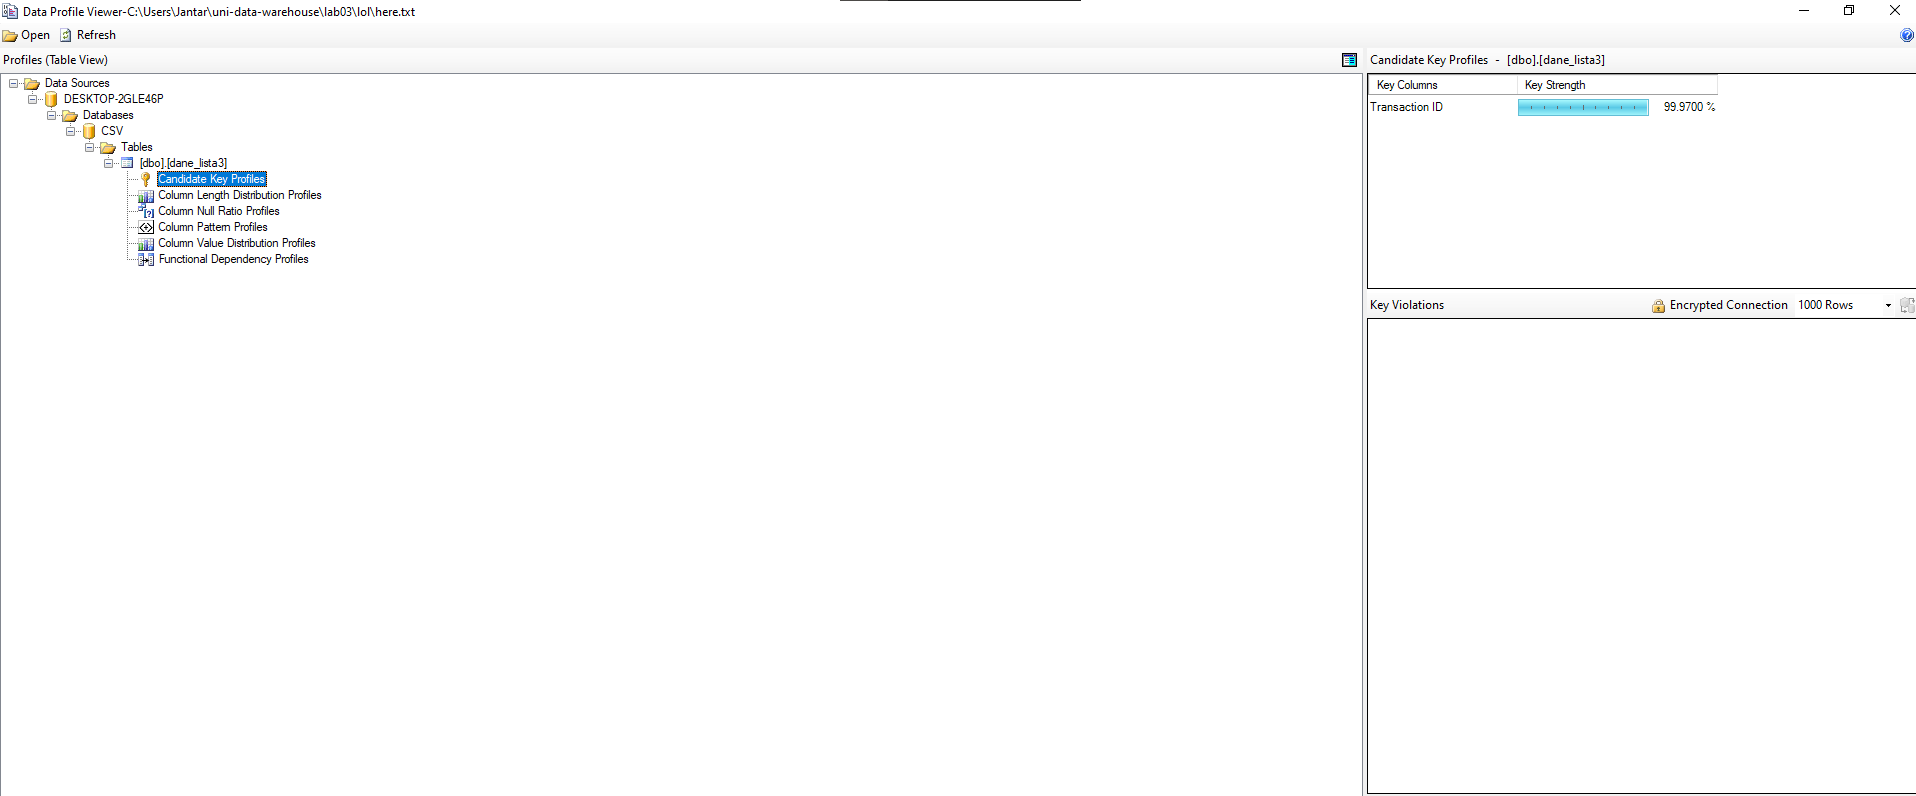
\includegraphics[width=1.0\textwidth]{images/ssis_1.png}
  \caption{Profil kolumny kandydującej}
\end{figure}

\begin{figure}[H]
  \centering
  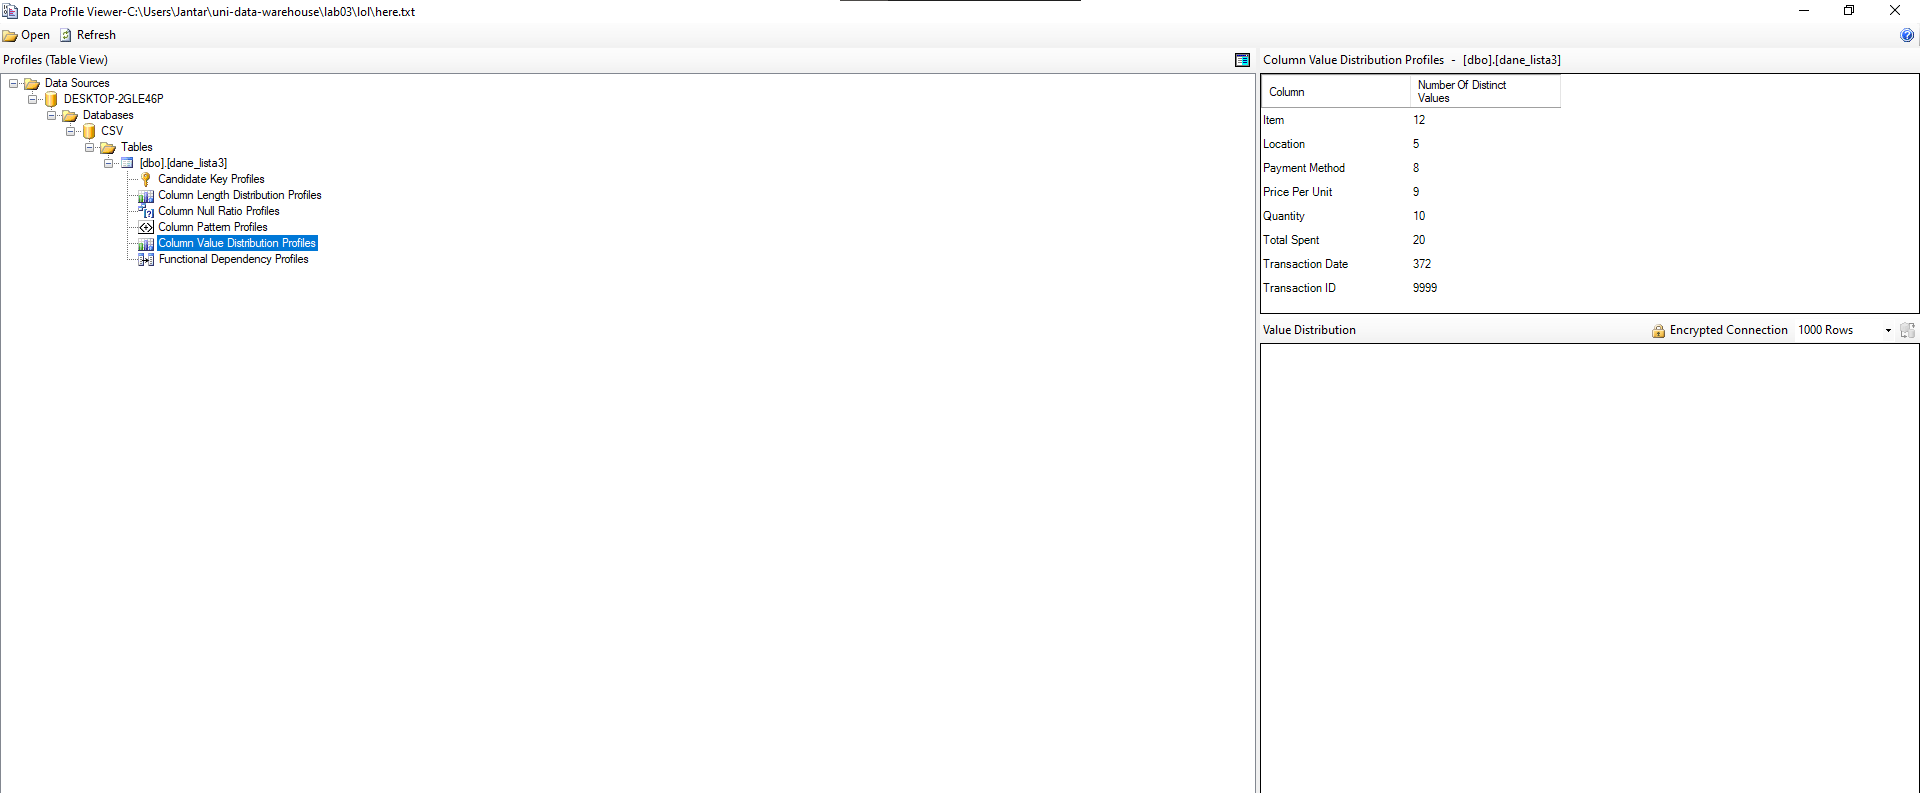
\includegraphics[width=1.0\textwidth]{images/ssis_2.png}
  \caption{Liczba unikatowych wartości w kolumnach}
\end{figure}

Z powodu problemów technicznych resztę analizy przeprowadzono używając \textit{Pythona} oraz bibliotek \textit{Pandas} i \textit{ydata\_profiling}.

\subsection{Transaction ID}

\begin{figure}[H]
  \centering
  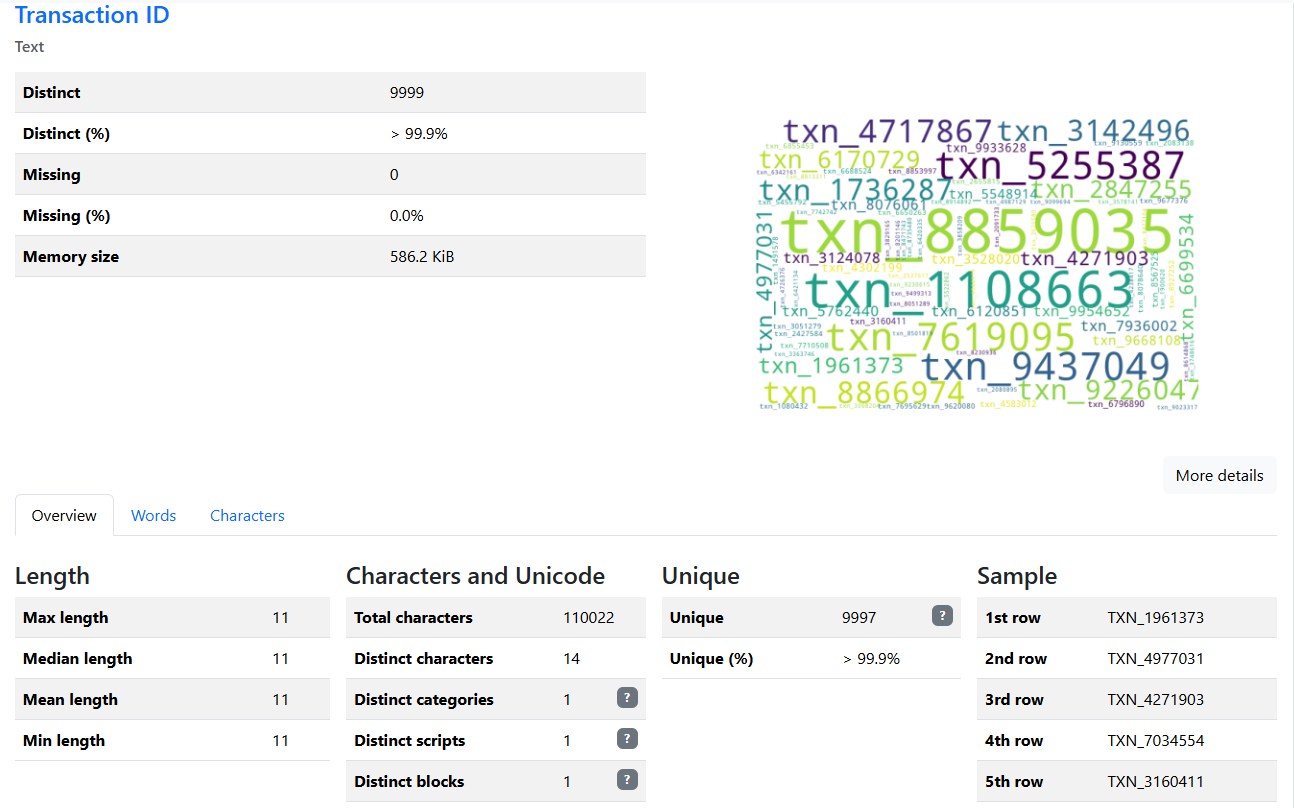
\includegraphics[width=0.65\textwidth]{images/py_1.png}
  \caption{Profil kolumny \textit{Transaction ID}}
\end{figure}

Tak jak też wywnioskowano wcześniej, jest to jedyna kolumna nadająca się na klucz kandydujący. Są w niej tylko 3 duplikaty. Zawsze ma też tą samą długość - 11 znaków.

\subsection{Item}

\begin{figure}[H]
  \centering
  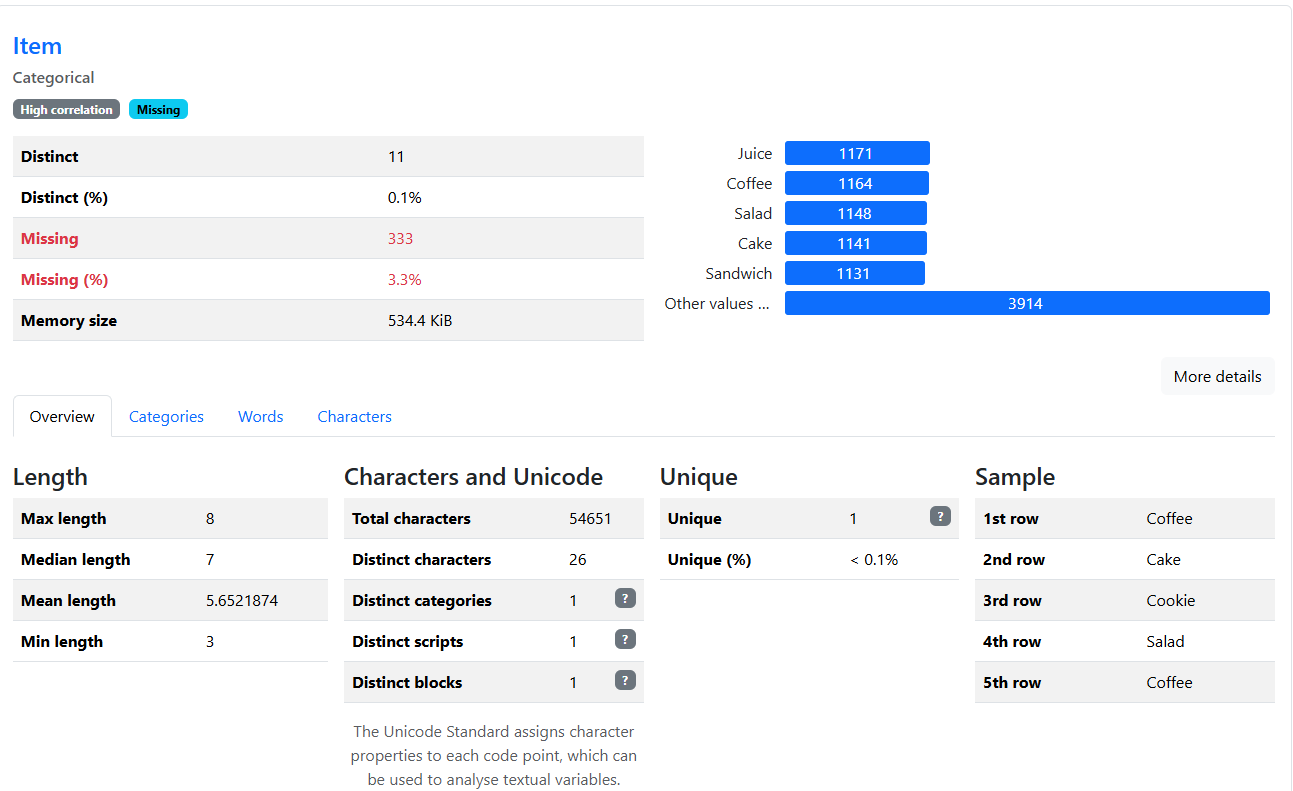
\includegraphics[width=0.65\textwidth]{images/py_2.png}
  \caption{Profil kolumny \textit{Item}}
\end{figure}

Kolumna jest kategoryczna i przypisuje transakcjom kategorię kupionego towaru. W 3.3\% wierszy brakuje wartości. Dodatkowo w 3.4\% to \textit{UNKNOWN}. 

\subsection{Quantity}

\begin{figure}[H]
  \centering
  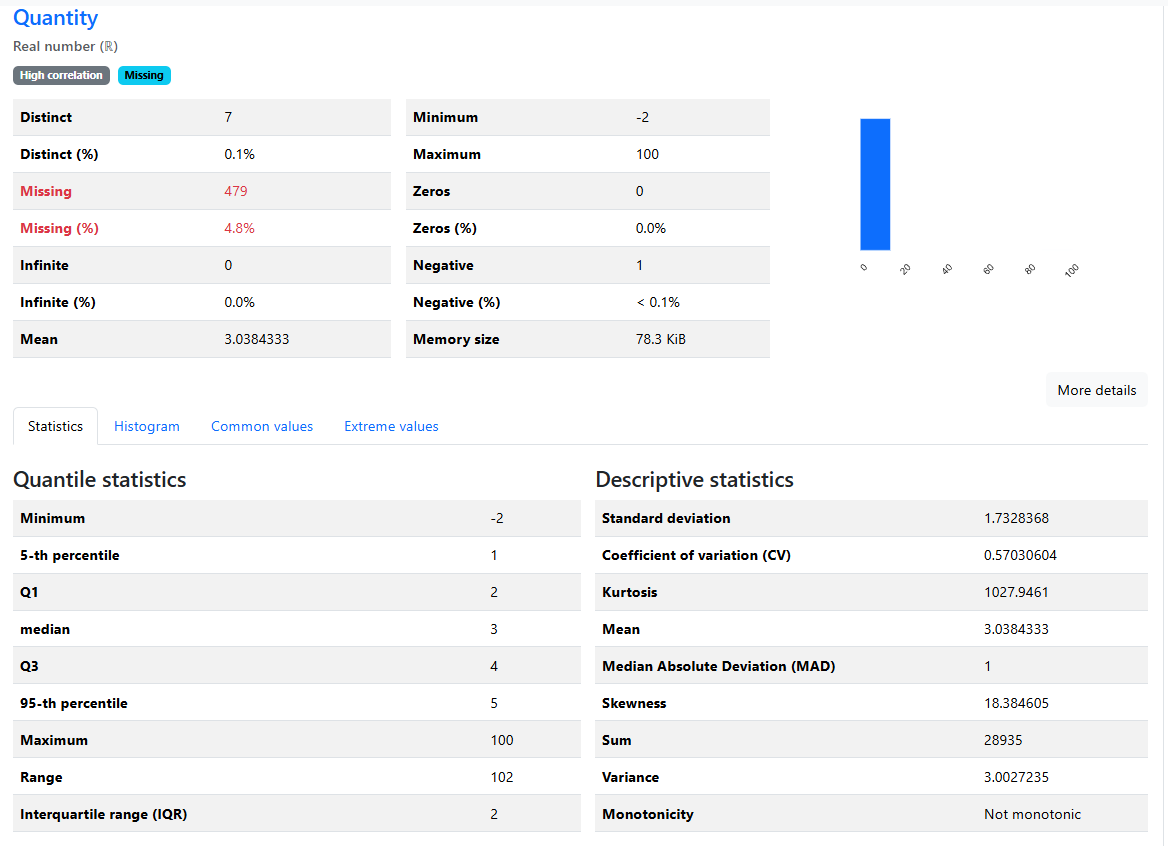
\includegraphics[width=0.65\textwidth]{images/py_3.png}
  \caption{Profil kolumny \textit{Quantity}}
\end{figure}

W kolumnie występują anomalnie. Zdarzyła się raz wartość ujemna: -2. Zdarzyła się raz wartość 100, znacznie przekraczająca poza zakres innych (1-5), ale być może dozwolona. Brakuje danych w 4.8\% wierszy. Wartości standardowe, czyli od 1 do 5 włącznie, występują z podobną częstością.

\subsection{Price Per Unit}

\begin{figure}[H]
  \centering
  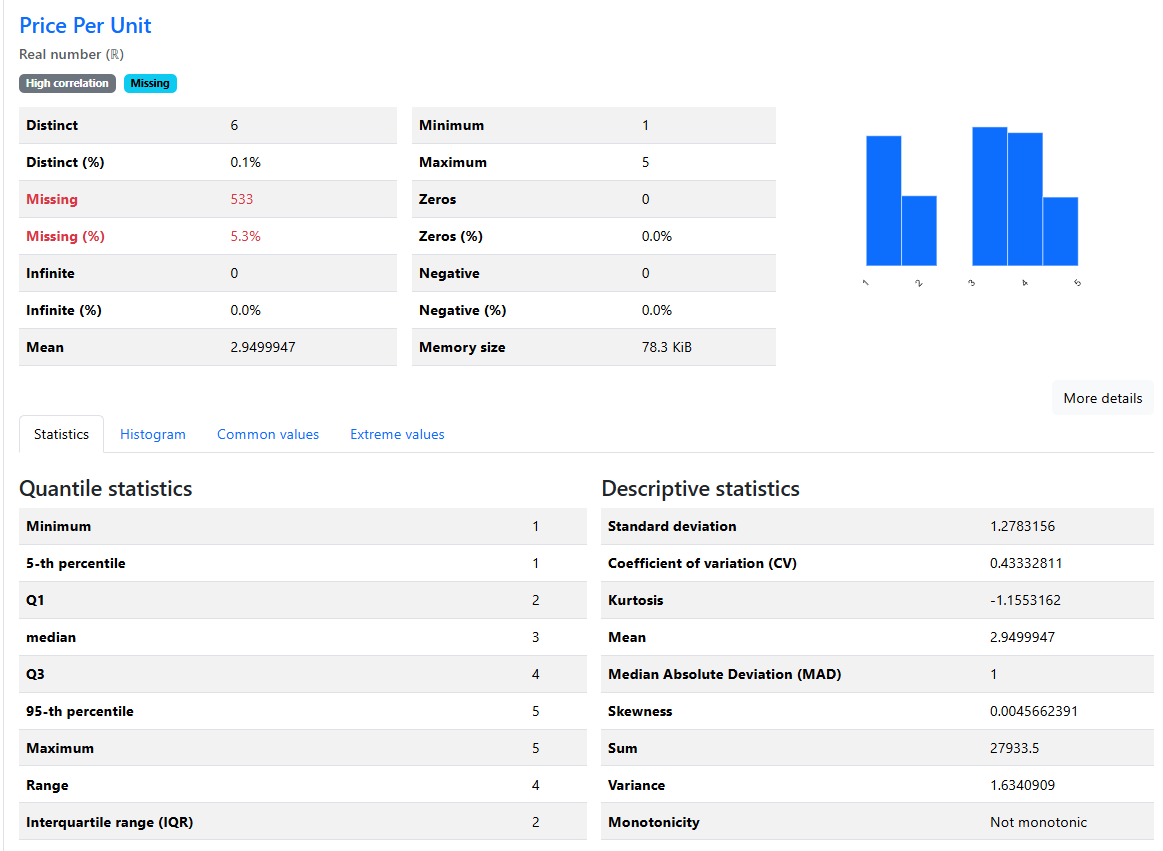
\includegraphics[width=0.65\textwidth]{images/py_4.png}
  \caption{Profil kolumny \textit{Price Per Unit}}
\end{figure}

Kolumna w większości składa się z liczb całkowitych, ale 11.3\% wartości to jedyne z wartością po przecinku. Wszystkie wynoszą dokładnie 1,5. Brakuje wartości dla 5.3\%. Standardowe i jedyne poza brakującymi wartości to liczby całkowite od 1-5 oraz 1,5. Najczęściej występuje wartość 3.

\subsection{Total Spent}

\begin{figure}[H]
  \centering
  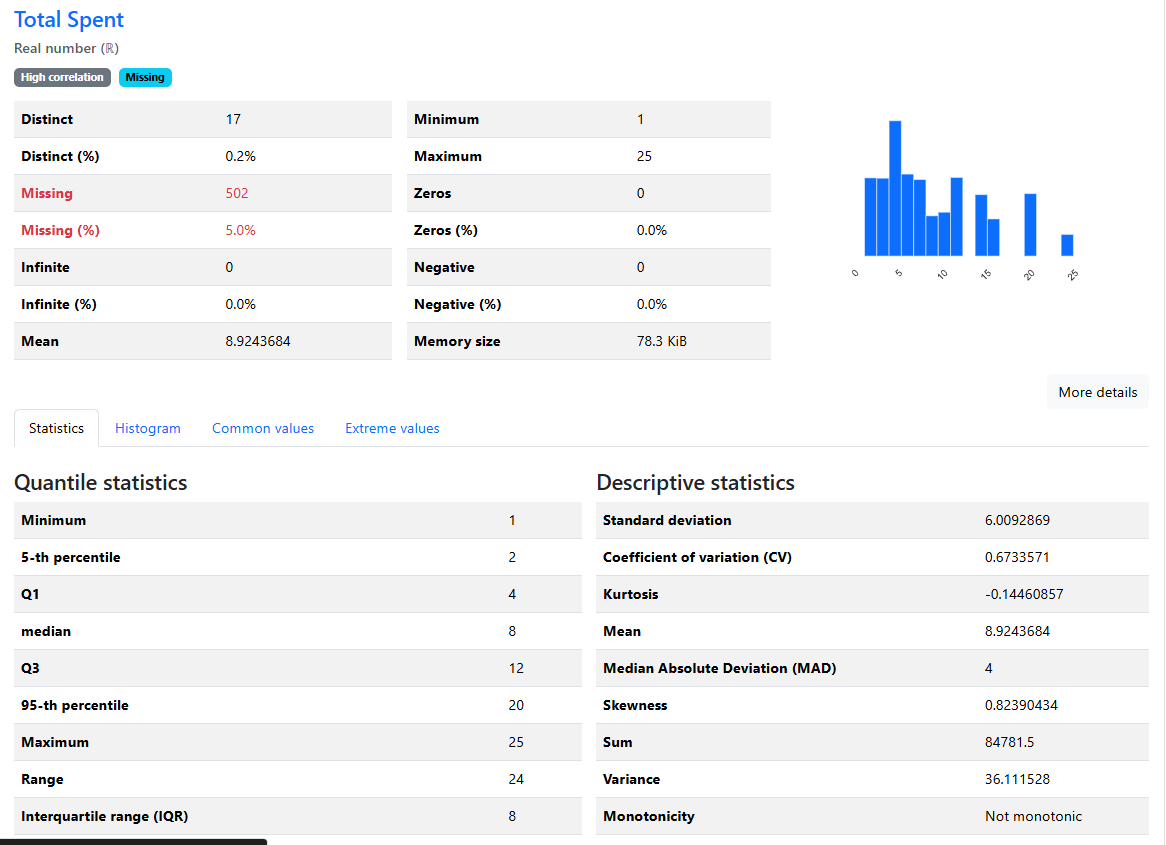
\includegraphics[width=0.65\textwidth]{images/py_5.png}
  \caption{Profil kolumny \textit{Total Spent}}
\end{figure}

Brakuje 5.02\% wartości. Przedział to liczby od 1 do 25 (ale tylko 17 z nich jest w danych). Większość wartości to liczby całkowite, ale występują też wielokrotności 1,5, sugerując, że cena 1,5 w Price Per Unit nie jest żadną anomalią. Najczęściej występuje wartość 6. Większość wartości jest bliżej początku rozkładu niż końca.

\subsection{Payment Method}

\begin{figure}[H]
  \centering
  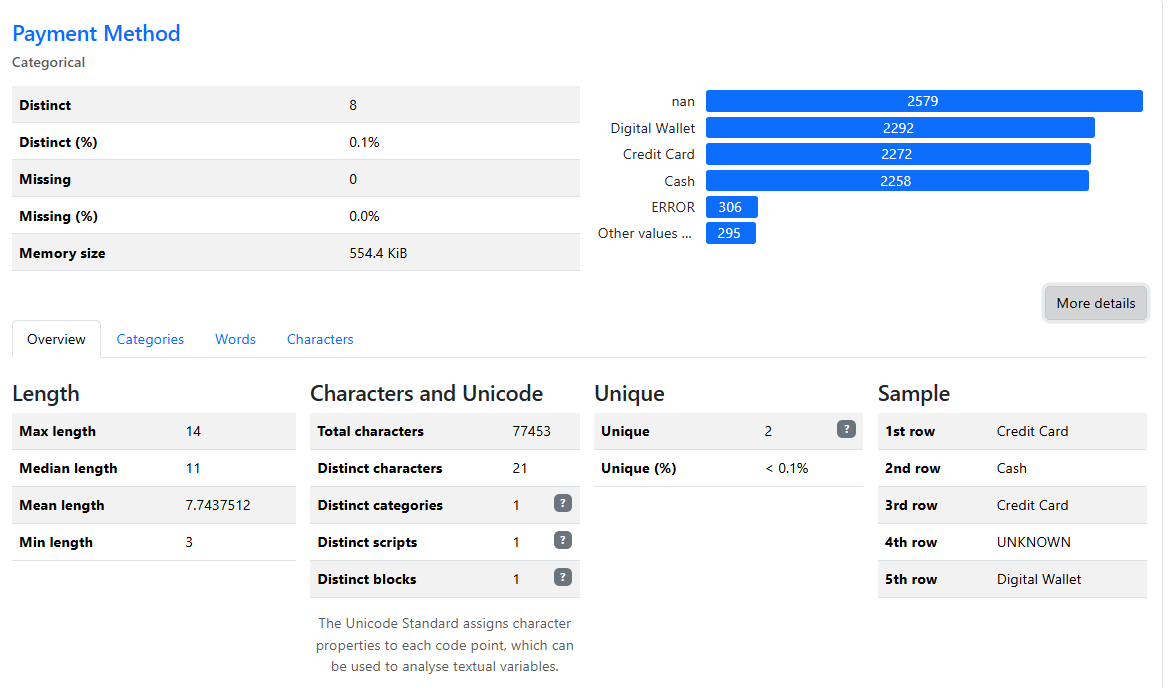
\includegraphics[width=0.65\textwidth]{images/py_6.png}
  \caption{Profil kolumny \textit{Payment Method}}
\end{figure}

Niepoprawne to 31,78\% całości - połaczenie \textit{nan}, \textit{ERROR} i \textit{UNKNOWN}. Oczywiście przy odczytywaniu karty mogą zdarzać się błędy, ale wtedy transakcje raczej powinny być odrzucane i nie znajdować się w bazie danych. Dodatkowo 2 razy wystąpiły literówki - Digital Walle i CreditCard zamiast Digital Wallet i Credit Card (występujących znacznie częściej). Poprawne kategorie to Digital Wallet, Credit Card	i Cash.

\subsection{Location}

\begin{figure}[H]
  \centering
  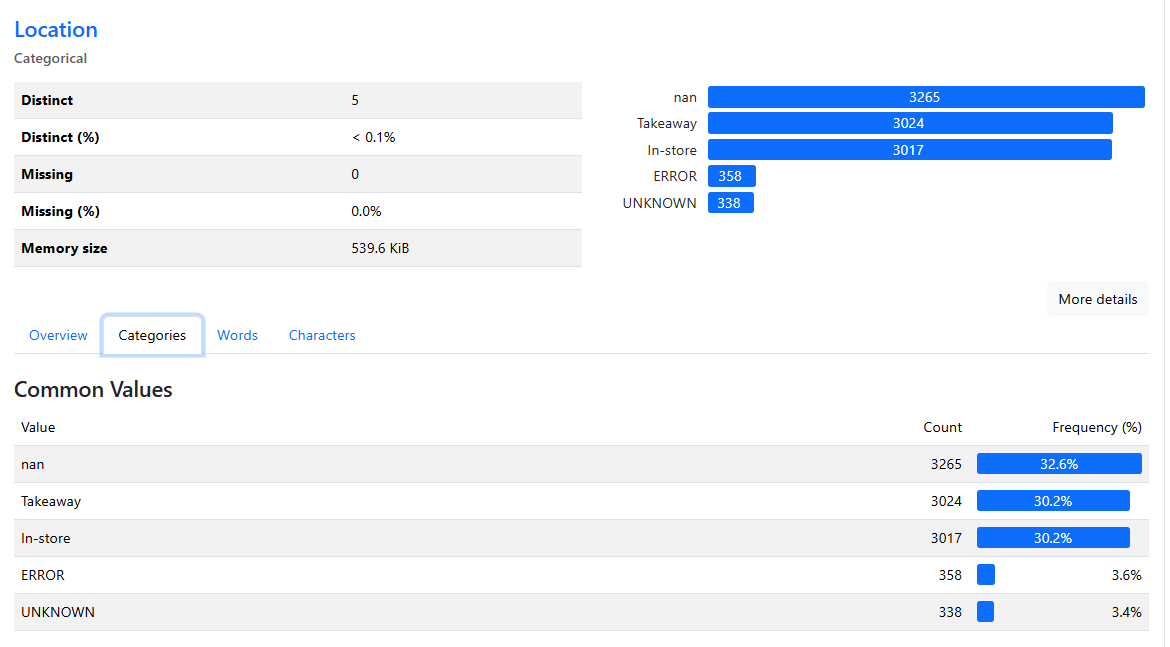
\includegraphics[width=0.65\textwidth]{images/py_7.png}
  \caption{Profil kolumny \textit{Location}}
\end{figure}

Podobnie jak poprzednio, wielu danych brakuje. Nan, ERROR i UNKNOWN występują z częstością 39,61\%. Poza tym, 2 poprawne kategorie to Takeaway lub In-store.

\subsection{Transaction Date}

\begin{figure}[H]
  \centering
  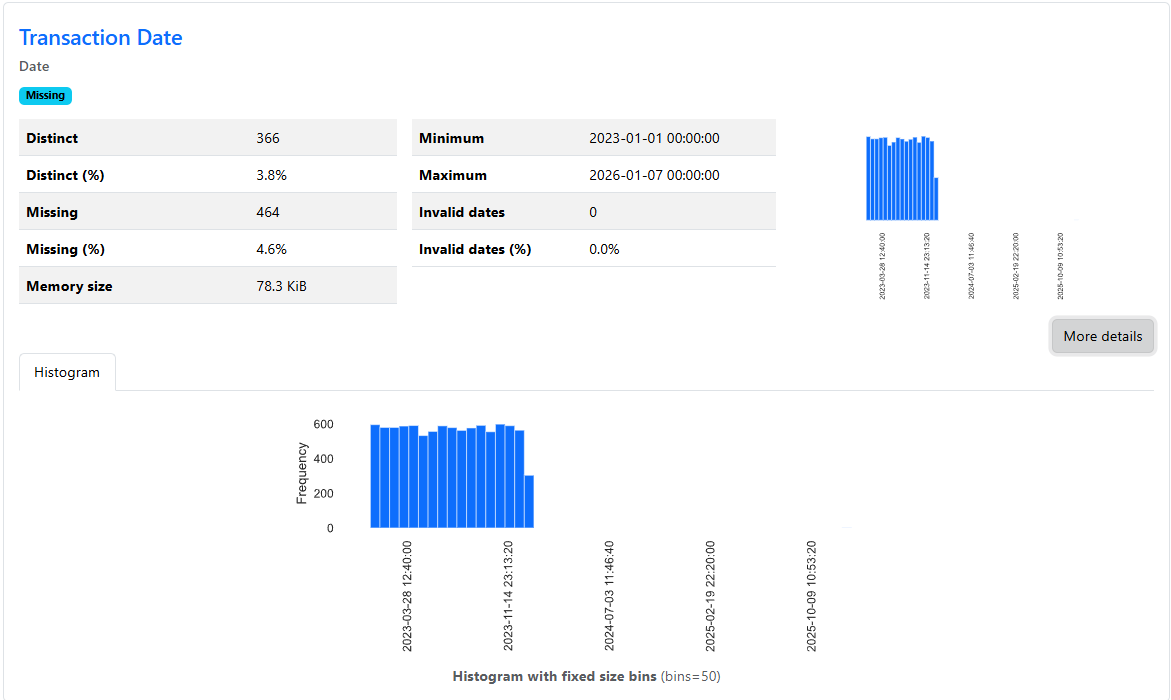
\includegraphics[width=0.65\textwidth]{images/py_8.png}
  \caption{Profil kolumny \textit{Transaction Date}}
\end{figure}

Przez jedną literówkę w danych zakres wydaje się być od 2023-01-01 do 2026-01-07. Rzeczywiście jednak dane są od 2023-01-01 do 2023-12-31, a wystąpiła literówka w 2026 i rok powinien zostać zmieniony na 2023. Poza tym rozkład jest dość równomierny, jedynie w grudniu jest wyraźny spadek. Brakuje 4,6\% wartości.

\subsection{Przykład interakcji}

\begin{figure}[H]
  \centering
  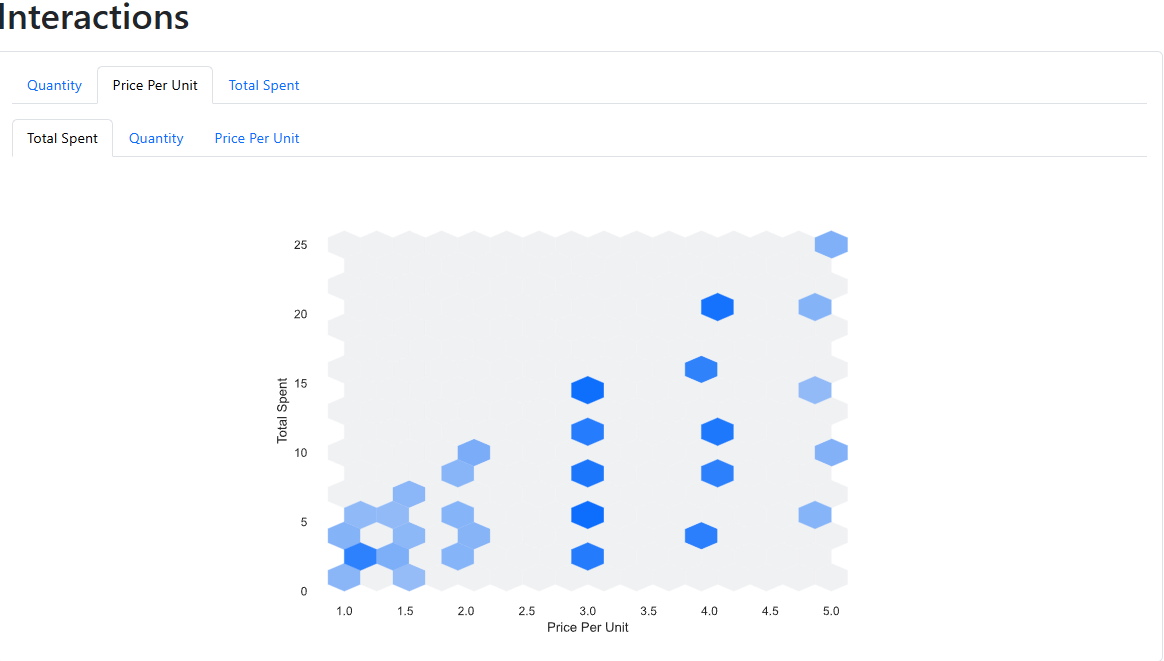
\includegraphics[width=0.65\textwidth]{images/py_interactions_example.png}
  \caption{Przykład interakcji między Price Per Unit a Total Spent}
\end{figure}

Jak widać, występuje pozytywna korelacja miedzy Price Per Unit a Total Spent.

\printbibliography

\end{document}